

\fancypagestyle{miEstilo501}{
   \lhead{5.1 Arquitectura de la aplicación}
   \rhead{Página \thepage}
   \lfoot{}
   \cfoot{}
   \rfoot{}
}

\pagestyle{miEstilo501}


\subsection{Arquitectura de la aplicación}

Esta aplicación consta de una \textbf{arquitectura basada en microservicios}. Una arquitectura de microservicios \cite{ref25} consta de una colección de servicios autónomos y pequeños. Los servicios son independientes entre sí y cada uno debe implementar una funcionalidad de negocio individual.

En cierto modo, los microservicios son la evolución natural de las arquitecturas orientadas a servicios aunque con ciertas diferencias.

\newpage

\textbf{¿Por qué se ha utilizado esta arquitectura?}

En primer lugar, se ha realizado una descomposición de los principales componentes necesarios para construir la aplicación, y se ha observado que hay funcionalidades independientes que se pueden comunicar entre sí para integrarse en la aplicación. Esto aporta una gran serie de ventajas respecto a un diseño monolítico \cite{ref26} como las siguientes:

\begin{itemize}
\item \textbf{Implementaciones independientes}: Es posible actualizar un servicio sin volver a implementar toda la aplicación y revertir o poner al día una actualización si algo va mal. Las correcciones de errores y las publicaciones de características son más fáciles de administrar y entrañan menos riesgo, por lo tanto, facilitan el mantenimiento de este software.

\item \textbf{Desarrollo independiente}: Cada microservicio se ha ido desarrollando a lo largo de una iteración y de forma independiente al resto. Esto ha agilizado bastante la tarea, ya que las modificaciones y errores no se retropropagaban.

\item \textbf{Fácil escalabilidad}: Cada microservicio puede ser escalado de forma independiente al resto. Por ejemplo, en el caso de que sea necesario escalar la detección de objetos en imágenes, bastaría con replicar el microservicio de detección de objetos y balancear las peticiones entre ellos.

\item \textbf{Fácil integración y alta cohesión}: Un sistema de microservicios se puede integrar y adaptar a casi cualquier sistema. Por ejemplo, en el caso de que quisiera añadir un sistema multicámara a la aplicación, bastaría con añadir una nueva capa superior de abstracción sobre el software desarrollado y se integraría perfectamente.
\end{itemize}

Basándome en esta arquitectura basada en microservicios, se ha diseñado el siguiente sistema (ver figura \ref{img:arquitectura}).

\newpage

\begin{figure}[h]
	\centering
	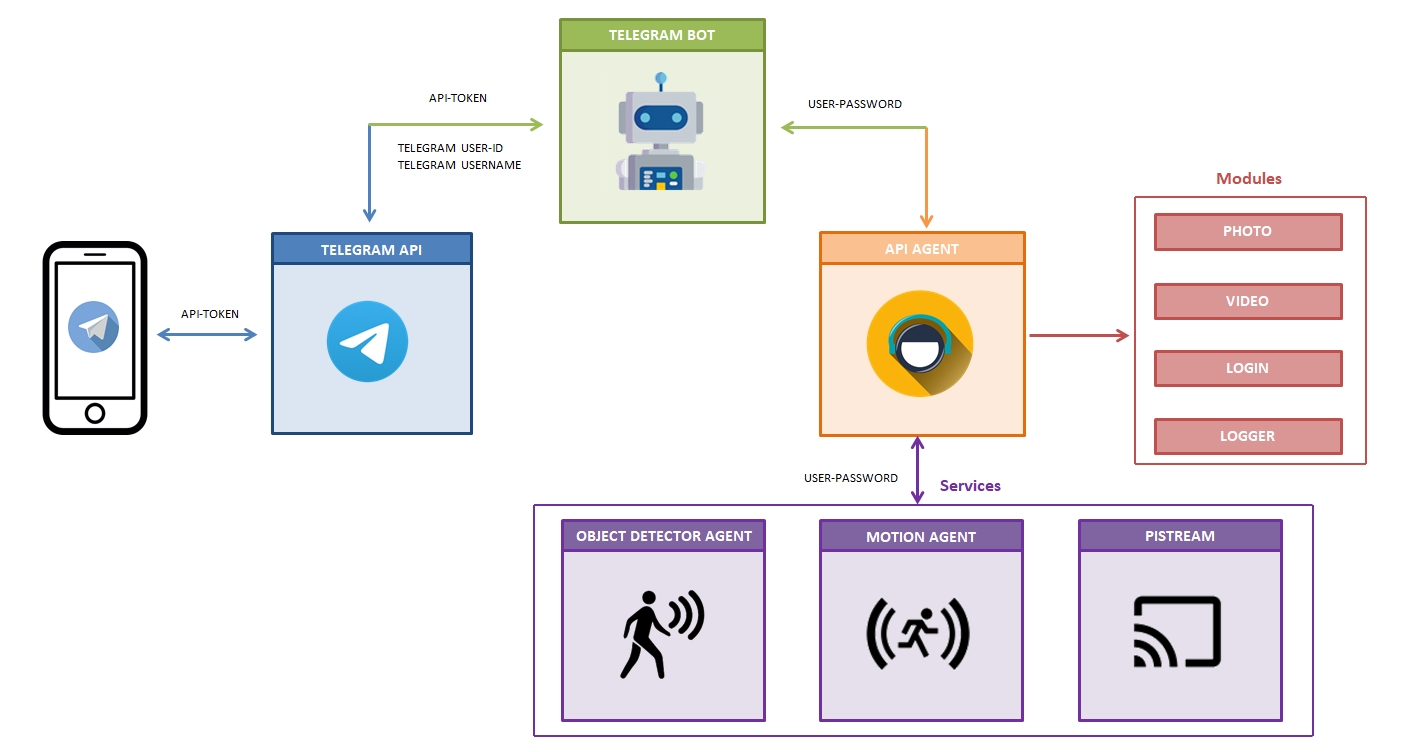
\includegraphics[scale=0.4]{images/23}
	\caption{Arquitectura de la aplicación}
	\label{img:arquitectura}
\end{figure}

En primer lugar tenemos los \textbf{módulos} de la aplicación (ver figura \ref{img:modulos}) que implementan un conjunto de funcionalidades para comunicarse con el módulo hardware de la cámara de la Raspberry PI, autenticación y logs.

\begin{figure}[h]
	\centering
	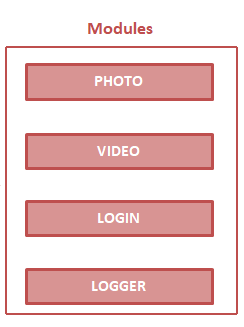
\includegraphics[scale=0.4]{images/24}
	\caption{Módulos de la aplicación}
	\label{img:modulos}
\end{figure}

A continuación tenemos el \textbf{API agent} (ver figura \ref{img:api}). Este es un servicio web que inicia la API que conecta con el resto de módulos de la aplicación.

\begin{figure}[h]
	\centering
	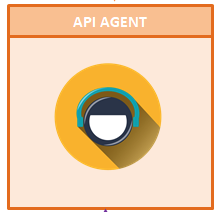
\includegraphics[scale=0.35]{images/25}
	\caption{API agent}
	\label{img:api}
\end{figure}

\newpage

Esta API importa y hace uso de los módulos de la aplicación. 

\begin{figure}[h]
	\centering
	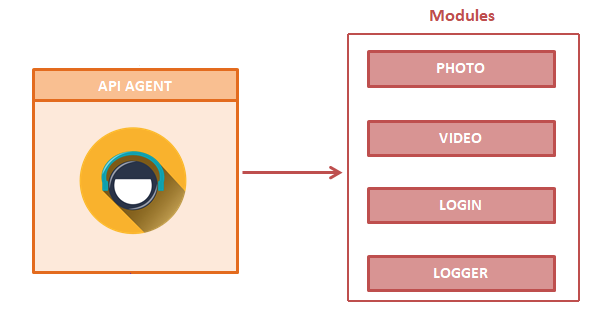
\includegraphics[scale=0.35]{images/27}
	\caption{Conexión entre la API y los módulos}
	\label{img:conexionapimodulos}
\end{figure}

Por otra parte, tenemos un conjunto de servicios que se inician de forma independiente y proporcionan las funcionalidades de detección de objetos en imágenes, detección de movimiento y servicio de streaming.

\begin{figure}[h]
	\centering
	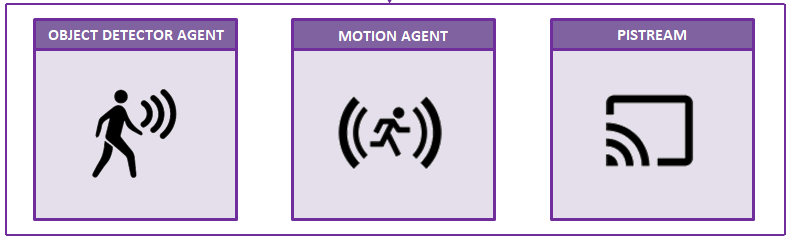
\includegraphics[scale=0.35]{images/26}
	\caption{Servicios de la aplicación}
	\label{img:serviciosaplicacion}
\end{figure}

La API está conectada con todo este conjunto de servicios y tiene la capacidad de poder gestionarlos.

\begin{figure}[h]
	\centering
	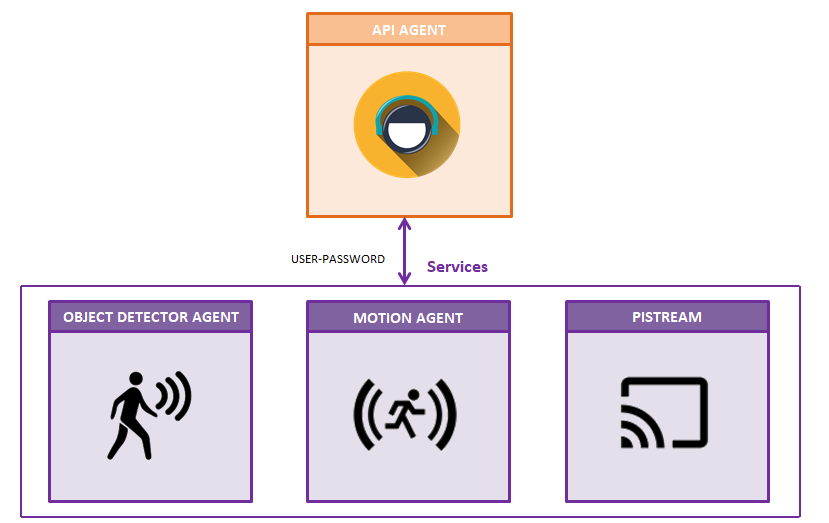
\includegraphics[scale=0.35]{images/28}
	\caption{Conexión entre los servicios y la API}
	\label{img:conexionserviciosapi}
\end{figure}

En la figura \ref{img:conexionmodulosserviciosapi} podemos ver, como quedan unidos todos estos componentes entre sí.

\newpage


\begin{figure}[h]
	\centering
	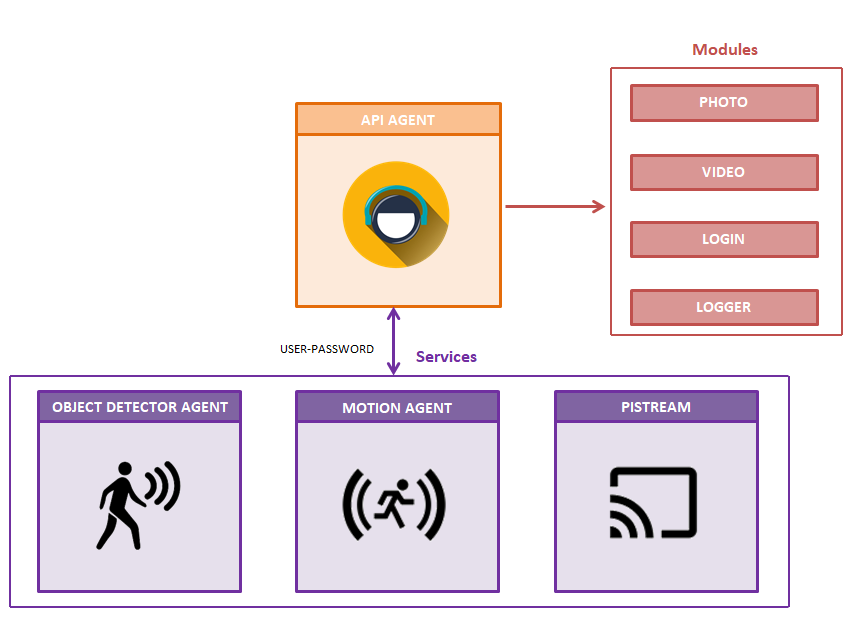
\includegraphics[scale=0.35]{images/35}
	\caption{Conexión de módulos y servicios con la API}
	\label{img:conexionmodulosserviciosapi}
\end{figure}

El siguiente componente es el \textbf{bot de Telegram}. Este bot es un proceso que se ejecuta junto a la API, cuyo objetivo es conectar la API de telegram con la API de la aplicación.

\begin{figure}[h]
	\centering
	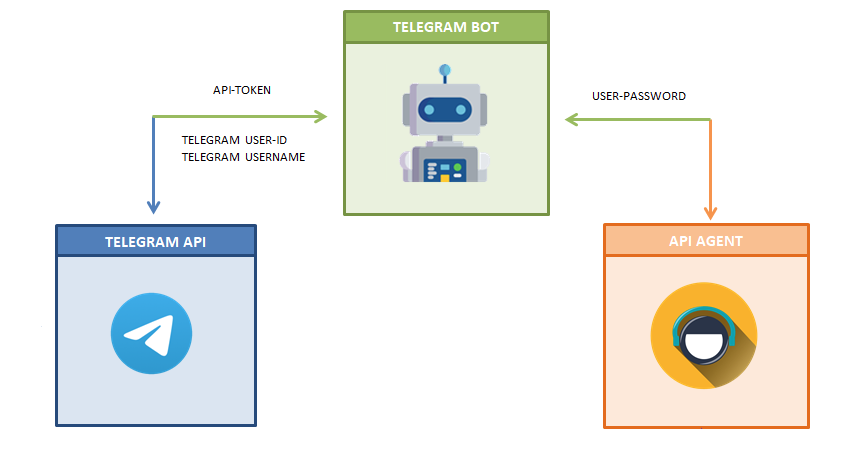
\includegraphics[scale=0.35]{images/34}
	\caption{Conexión entre el bot de telegram y la API}
	\label{img:conexionbotapitelegram}
\end{figure}

Finalmente, el usuario puede interactuar con la aplicación (\texttt{SIVIRA}), haciendo uso de la aplicación multiplataforma \texttt{Telegram}, usando el bot que se ha creado.

\begin{figure}[h]
	\centering
	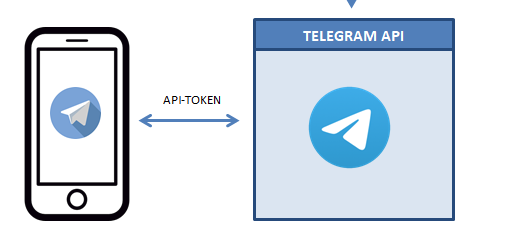
\includegraphics[scale=0.35]{images/33}
	\caption{Conexión entre el usuario y la aplicación}
	\label{img:usuariotelegram}
\end{figure}

\newpage
